\chapter{Réseaux programmables avec SDN}

On cherche à concevoir une architecture plus adaptée aux enjeux de la communication de l'actualité discutés dans le chapitre 1. Cette problématique a amené scientistes et les ingénieurs impliqués à concevoir \gls{sdn}. \gls{sdn} est un nouveau \glslink{paradigme}{paradigme} réseau qu'on est actuellement en cours de développer pour adapter l'infrastructure existante à ce nouveau scénario.
Le but de ce chapitre est de (re)définir SDN et de présenter en quoi SDN répond aux besoins explicités dans le chapitre 1.
%Ce chapitre répond aux questions : Qu'est-ce que SDN ? Qu'est-ce que cela propose ?
Le chapitre propose aussi un point sur la situation de SDN, en présentant les organisations qui l'adopte et ce qui a été développé en terme de standards et protocoles.

\section{Séparation de l'intelligence (contrôle) de la commutation (flux de données)}

%Having recognized the problem, the networking commu- nity is hard at work developing programmable networks, such as GENI [1] a proposed nationwide research facility for experimenting with new network architectures and dis- tributed systems. These programmable networks call for programmable switches and routers that (using virtualiza- tion) can process packets for multiple isolated experimen- tal networks simultaneously.
Ayant adressé cette problématique, la communauté réseau fait beaucoup d'efforts pour le développement des réseaux programmables. Ces réseaux programmables utilisent des switches et des routeurs programmables qui peuvent traiter des paquets pour des multiples réseaux expérimentaux  à la fois, grâce à la \gls{virtualisation}. \cite{OpenFlowStanfordOssification} Divers projets pour les réseaux programmables, comme NETCONF \cite{NETCONF}, Ethane \cite{Ethane}, GENI \cite{GENI} etc. ont été réalisés et en ont servi de base pour ce paradigme qu'on développe et supporte aujourd'hui : \gls{sdn}. 

%SDN is described in this article with the Open Networking Foundation (ONF) [1] definition: “In the SDN architecture, the control and data planes are decoupled, network intelli- gence and state are logically centralized, and the underlying network infrastructure is abstracted from the applications.”

SDN est défini au long de cette étude  selon \gls{onf} : Dans l'architecture SDN, les plans de contrôle et de données sont découpés, l'intelligence et l'état du réseau sont logiquement centralisés, et l'infrastructure du réseau est donc abstraite des applications. \cite{SDNNewNormONFExecutiveSummary}


%The control plane is responsible for configuration of the node and programming the paths that will be used for data flows. Once these paths have been determined they are pushed down to the data plane. Data forwarding at the hardware level is based on this control information.

[déf plan de contrôle => intelligence, logique, implémentation des protocoles]. [Déf plan de donnés, flux, commutation]
Le plan de contrôle est responsable pour la configuration d'un nœud et pour la programmation des chemins qui seront utilisés par les flux de données. Le plan de donnés fourni au hardware les informations nécessaires à la commutation. \cite{ImplementationChallengesForSDNBackground}

\clearpage


Dans l'architecture réseau traditionnellement déployée, chaque nœud contient un plan de contrôle et un plan de données à l'intérieur du même matériel. L'ossification d'internet discuté dans le chapitre 1 est largement attribuée à ce fort couplage entre les deux plans provocant que toutes les décisions sur les flux de donnés soient embarqués dans chaque élément réseau. La manque d'une interface de contrôle commune à tous les dispositifs complique toute évolution que cela soit un simple changement de configuration ou le développement d'une nouvelle application.



%As mentioned previously, the so-called Internet “ossifica- tion” [2] is largely attributed to the tight coupling between the data– and control planes which means that decisions about data flowing through the network are made on-board each network element. In this type of environment, the deployment of new network applications or functionality is decidedly non- trivial, as they would need to be implemented directly into the infrastructure. Even straightforward tasks such as config- uration or policy enforcement may require a good amount of effort due to the lack of a common control interface to the various network devices.

Avec SDN, on propose la séparation de ces deux éléments. Un contrôleur centralisé est commun à tous les équipements qui passent à contenir seulement le plan de donnés un plus d'un module de communication. 
Dans l'image ci-dessous on voit un schéma montrant un nœud du point de vu de ces deux modèles, ensuite on affiche un image présentant l'ensemble de l'architecture dans les deux cas.

\begin{figure}[!h] %on ouvre l'environnement figure
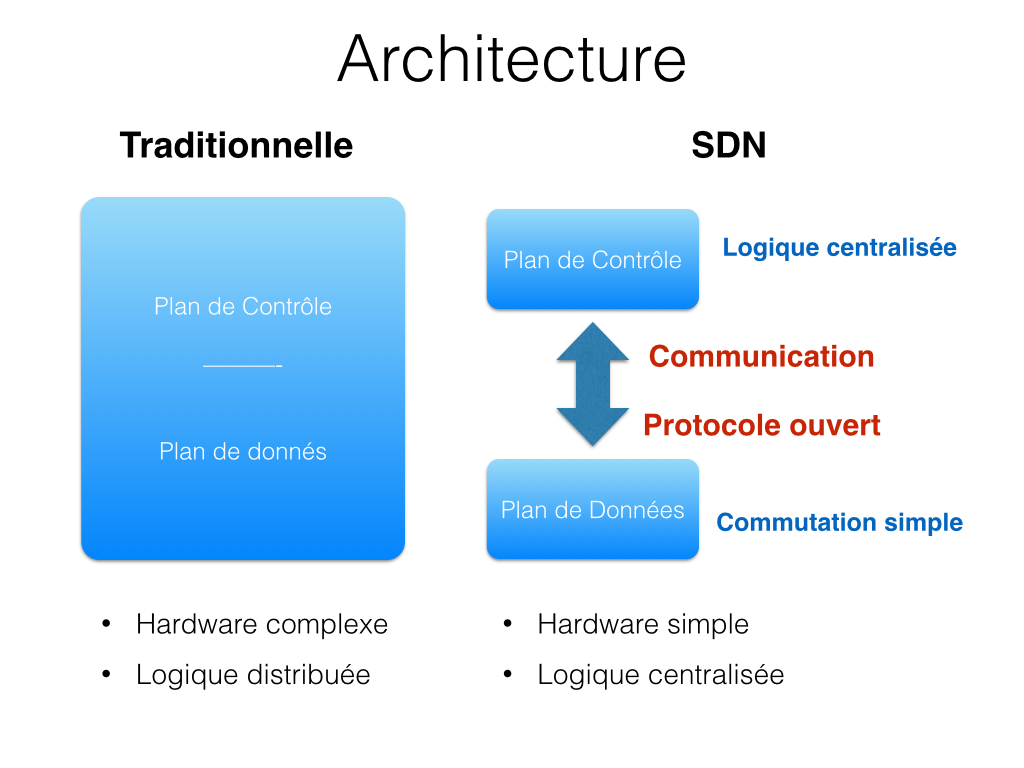
\includegraphics[width=15cm]{images/ComparaisonArchis.png} %ou image.png, .jpeg etc.
\caption{ Un nœud dans l'Architecture Traditionnelle et SDN} %la légende
\label{imgNodesArchi} %l'étiquette pour faire référence à cette image
\end{figure} %on ferme l'environnement figure



\begin{figure}[!h] %on ouvre l'environnement figure
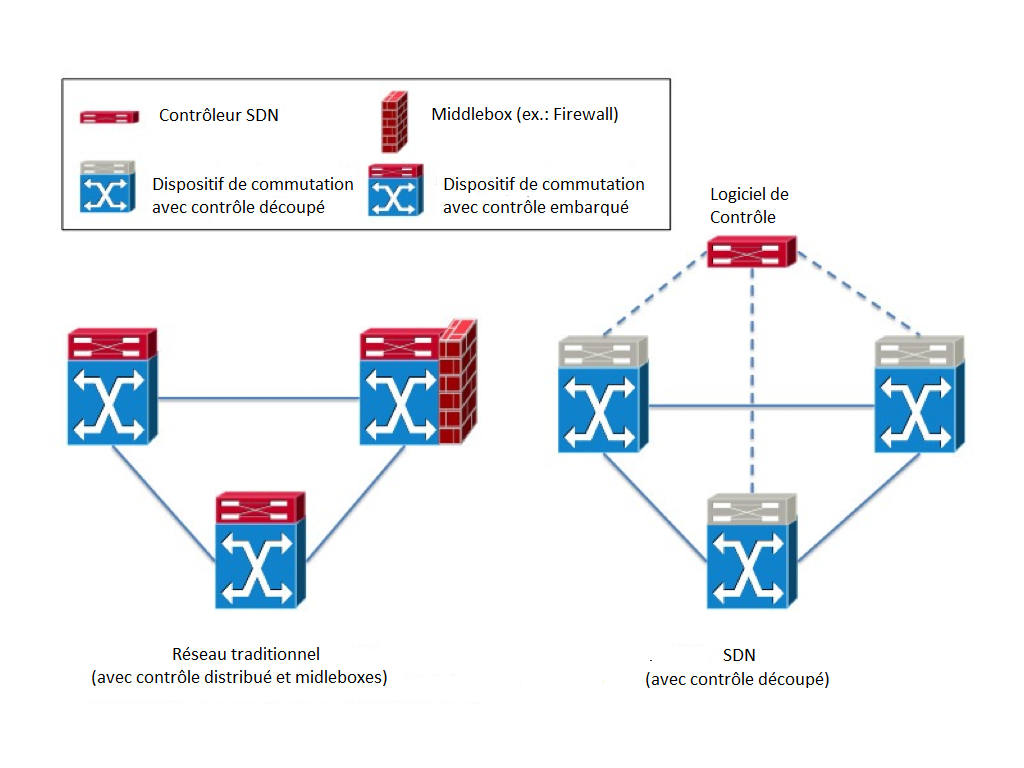
\includegraphics[width=15cm]{images/TraditionalVsSDN.png} %ou image.png, .jpeg etc.
\caption{ L'ensemble de l'Architecture Traditionnelle et SDN \cite{SurveySDNArchi}} %la légende
\label{imgOverviewArchi} %l'étiquette pour faire référence à cette image
\end{figure} %on ferme l'environnement figure

\clearpage


\section{Dispositifs de commutation}
%The basic idea is simple: we exploit the fact that most modern Ethernet switches and routers contain flow-tables (typically built from TCAMs) that run at line-rate to im- plement firewalls, NAT, QoS, and to collect statistics. While each vendor’s flow-table is different, we’ve identified an in- teresting common set of functions that run in many switches and routers. OpenFlow exploits this common set of func- tions.

SDN profite du fait que la majorité des switches et routeurs existants contiennent des tableaux de flux qui exécutent à une fréquence ligne pour implémenter leurs protocoles et collecter des statistiques.

\section{Contrôleur}
Controllers. A controller adds and removes flow-entries from the Flow Table on behalf of experiments. For example, a static controller might be a simple application running on a PC to statically establish flows to interconnect a set of test computers for the duration of an experiment. In this case the flows resemble VLANs in current networks— providing a simple mechanism to isolate experimental traffic from the production network. Viewed this way, OpenFlow is a generalization of VLANs.

\section{Un point sur la situation}
%\subsection{ONF}

%The Open Networking Foundation (ONF) is a non‑profit, user‑driven organization dedicated to accelerating the adoption of open Software‑Defined Networking (SDN). We view SDN as a disruptive approach to networking that will change how virtually every company with a network operates.

%Launched in 2011 by Deutsche Telekom, Facebook, Google, Microsoft, Verizon, and Yahoo!, ONF is a nonprofit organization dedicated to rethinking networking, and quickly and collaboratively bringing to market SDN standards and solutions. ONF is accelerating the delivery and commercialization of SDN and fostering a vibrant market of products, services, applications, customers, and users. 


Open Networking Foudation (\gls{onf}) et une organisation non-profit et axée sur l'utilisateur dédiée à l'accélération de l'adoption ouverte de SDN. Cette organisation voit SDN comme une approche réseau qui va changer comment opère chaque entreprise avec un réseau.
\gls{onf} a été initiée en 2011 par Deutsche Telekom, Facebook, Google, Microsoft, Verizon et Yahoo! dans le but de repenser en collaboration les réseaux informatiques et rapidement apporter au marché les solutions et les standards SDN. Avec la collaboration de  grands experts mondiaux, ONF accélère la commercialisation de SDN en favorisant un vif marché de produits, services, applications, clients et utilisateurs. ONF compte aujourd'hui avec plus de 100 entreprises membres collaboratives de tout taille et variété. \cite{ONFOverview}


%The strong support from industry, research, and academia that the Open Networking Foundation (ONF) and its SDN proposal, OpenFlow, has been able to gather is quite impres- sive. The resulting critical mass from these different sectors has produced a significant number of deliverables in the form of research papers, reference software implementations, and even hardware. So much so that some argue that OpenFlow’s SDN architecture is the current SDN de-facto standard. In line with this trend, the remainder of this section focuses on OpenFlow’s SDN model. 

%The Open Network Foundation (ONF) [3] has been trying to standardize the OpenFlow protocol. As the control plane abstracts network applications from underlying hardware infrastructure, they focus on standardizing the inter- faces between: (1) network applications and the controller (i.e. northbound interface) and (2) the controller and the switching infrastructure (i.e., southbound interface) which defines the OpenFlow protocol itself. 

%\subsection{OpenFlow - Protocoles standardisés}
